\newpage

\section{Reproducing stylized facts with HMMs}
\label{Section: Stylized facts}


\textbf{Section structure:}
\begin{itemize}
    \item Consider moving data section to here
    \item Discuss why rolling estimation might be better than Bulla 2011 and Ryden 1998 - go over some the results where they did not get accuracte results - such as PED 1-3.
    \item Show estimated models
    \begin{itemize}
        \item Plot estimated models. Discuss certain smoothing procedures to improve models.
        \item \textbf{Draw this}. Plot first four moments to further see "fit"
        \item If possible here would be a nice place to put the 3d plot of distribution as a function of time
    \end{itemize} 
    \item Review stylized facts of GD
    \item Distributional properties
    \begin{itemize}
        \item DP2+DP3: Plot mean/std, skewness + kurtosis of absolute returns
        \item \textbf{Draw this} Show plot again for outlier corrected data. Note whether this is necessary.
    \end{itemize}
    \item Temporal properties
    \begin{itemize}
        \item Show calculations of plots for TP1+TP4 - very basic though.
        \item Start by showing ACF of full data and data split into subsamples to further motivate rolling models. Then show ACF of absolute returns of models in subsamples.
        \item TP2: Plot ACF of absolute returns. Consider also showing that ACF of squared returns is indeed smaller.
        \item TP3: Plot Taylor effect and explain procedure.
        
    \end{itemize}
    \item Current decoding/prediction is not really used for anything. Consider deleting or changing the analysis. Basing the section on smoothing probabilities in the rolling model might be better than showing predictions since this is what is used in forecasting in MPC framework.
\end{itemize}

As highlighted throughout section \ref{section: Data} the normal distribution provides a poor fit for financial returns. Furthermore, financial returns are characterised by a set of stylized facts. Researchers including Granger \& Ding (1995b), Cont (2001) and Malmsten \& Teräsvirta (2010) have found a variety of different stylized facts that are persistent across asset returns. In addition, Rýden et al. (1998) showed the how HMMs can reproduce most of the stylized facts, in which the analysis was rooted on daily returns of the S\&P 500. Rýden et al. (1998) found that most of the stylized facts could in fact be reproduced by a HMM, however, the slow decay characterising the  squared autocorrelation function of daily returns, which is of great importance in financial risk management, could not be reproduced satisfactorily. More recently, Nystrup (2017) showed promising results in terms of HMMs reproducing the the squared autocorrelation function, albeit not achieving a perfect fit. 

The data analyzed in this thesis encompass daily returns of the S\&P 500 stock index from 1960 to 2021. As such, the predominant amount of the time series data used by the above-mentioned authors, is represented in the data underlying this thesis. Despite the unanimity in the overall methodology of the studies conducted by the aforementioned authors there are differences in their respective objectives. For instance, Granger \& Ding (1995b) divided the time series data into ten subsamples of 1,700 observations, which corresponds to a little less than seven years. Granger \& Ding (1995b) worked under the assumption that it was likely that with such a long time span there could have been structural shifts in the datagenerating process. Using a similar approach, Rydén (1998) found that the estimated HMMs, including the number of states and the type of conditional distributions, changed considerably between the subsamples.

As such, this section will be reserved for training HMMs through the aforementioned MLE and JUMP methodology, after-which the corresponding models serve as subject for analysis of how well they reproduce the stylized facts. The methdology outlined in this section will take a great amount of inspiration from Granger \& Ding (1995), Rýden et al. (1998) as well as Nystrup (2017).

\subsection{Rolling estimation}
\label{Sec: rolling estimation}
Rýden et al. (1998) relied on a methodology in which a Gaussian HMM is estimated for ten subseries of a log return series generated from 17,000 daily observations from the S\&P 500 index. This methodology also closely follows the methodology originally put forward by Grangner \& Ding (1995b). In recent publications Bulla (2011) and Nystrup (2014) rely on estimating univariate HMMs through a rolling window of (1000 or 2000) trading days. This will result in ($\text{Number of observations} - 2000$) models being estimated, which thereby allows for capturing the time-varying nature of the HMMs' parameters. The advantage of Nystrup's methodology is the fact that the rolling window allows for gradually forgetting previous observations when estimation the models, whereas the subset methodology presented by Granger \& Ding estimates 10 unique HMMs from non-overlapping observations from the return series. 

As highlighted in section \ref{section: Data} this thesis relies on daily observations due to the favorable properties associated with early detection. The explanatory variable will be the daily returns of the S\&P 500 index, thereby making the results somewhat comparable to the aforementioned authors. It should be noted that it is not important whether the explanatory variable is tradeable as it will purely be used for signalling regime changes. Stock indices and yield spreads both serve as popular explanatory variables as they tend to lead the economy (Dungey et al, 2000). Essentially this means that stock indices and yield spreads will exhibit local maxima/minima approximately around the time of an economic regimes change. As such, both are suitable indicators, however, to increase comparability to the aforementioned literature, stock indices, and more precisely, the S\&P 500 index is preferred. 

As emphasized in section \ref{section: estimation}, this thesis aims at comparing the properties of the MLE and JUMP estimation procedure, in which a vital part of comparing and determining the most viable estimation methodology revolves around the methodology's capability of reproducing the stylized facts associated with asset returns. For this section the thesis will estimate 2-state univariate Gaussian HMMs through the MLE and JUMP methodology using a rolling window of XXXX trading days. That is, for each time step $t$ a HMM is estimated by the MLE and JUMP approach using the previous XXXX log returns, as the model parameters are stable at this length. Furthermore, the chosen window length makes it appropriate to compare results against those of Bulla (2011) and Nystrup (2014), albeit these authors neglect estimation the HMMs through the JUMP framework. After origination the rolling window moves one time period forward to $t+1$ iteratively. The choice of the number of trading days regarding the window length is based on the aforementioned authors which all select a rolling window length between 1000 and 2000 days. Essentially, the window length is a hyperparameter that can be tuned and the exact choice boils down to a trade-off relationship between bias and variance. A shorter rolling window will, all else equal, result in a faster adaption to changes in the underlying economic regimes but the estimate will be more noisy as fewer observations are used when deriving the parameters. This might result in the model adapting to "wrong" signal, which might affect the underlying trading strategy by decreasing risk-adjusted returns. A range of rolling window days have been tested and can be found in appendix XXX.

The results of the rolling parameter for the MLE and JUMP estimation of the 2-state Gaussian HMMs are shown in figure \ref{fig: MLE estimation rolling parameters} and \ref{fig: Jump estimation rolling parameters} respectively.

\begin{figure}[H] 
    \centering
    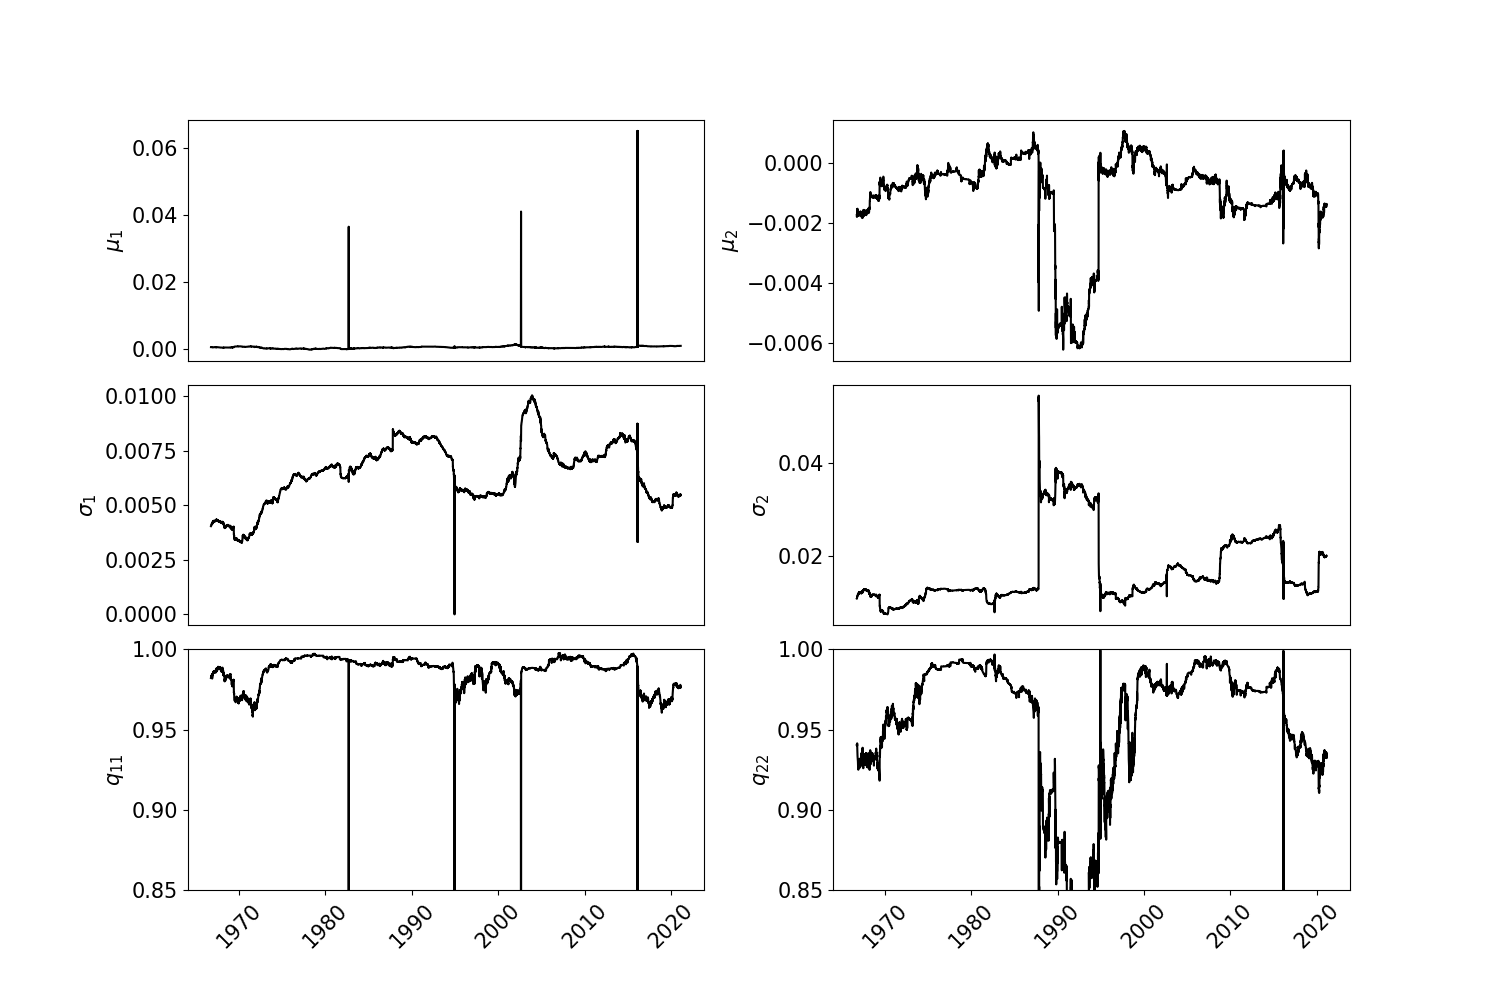
\includegraphics[width=1.0\textwidth]{analysis/stylized_facts/images/2-state MLE HMM rolling params.png}
    \caption{Rolling estimation based on the MLE approach. Parameters from a 2-state Gaussian HMM using a rolling window of 1700 days. The size of the estimation window is particularly visible in the bear state where $\sigma_2^2$ significantly increase after the financial crisis, and only drops back down to pre-crisis levels after approximately 1700 days.}
    \label{fig: MLE estimation rolling parameters} 
\end{figure}

\begin{figure}[H] 
    \centering
    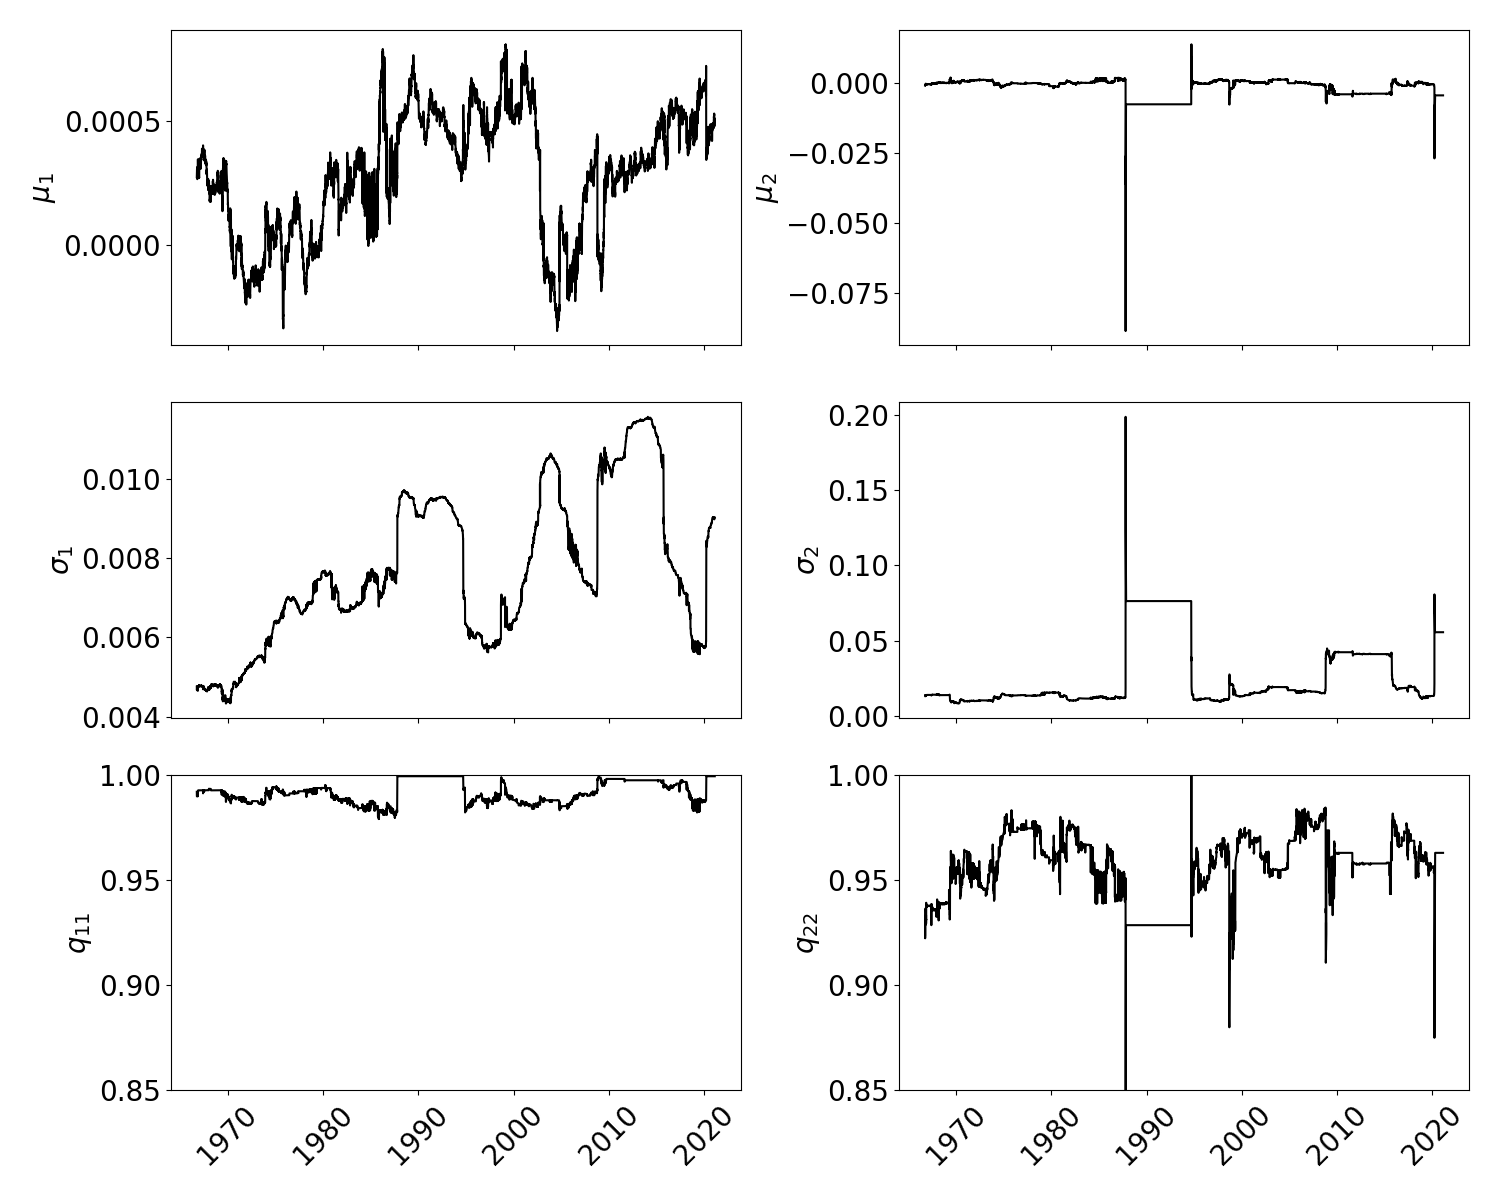
\includegraphics[width=1.0\textwidth]{analysis/stylized_facts/images/2-state JUMP HMM rolling params.png}
    \caption{Rolling estimation based on the JUMP approach. Parameters from a 2-state Gaussian HMM using a rolling window of XXX days.}
    \label{fig: Jump estimation rolling parameters} 
\end{figure}

From figure \ref{fig: MLE estimation rolling parameters} and \ref{fig: Jump estimation rolling parameters} it is evident that neither the mean nor variance parameters exhibit stationarity across time
for the 2-state Gaussian HMM regardless of whether the estimation procedure relies on MLE or JUMP. Starting with the MLE approach showcased in figure \ref{fig: MLE estimation rolling parameters} it becomes eveident that around the global financial crisis an interesting pattern emerges since $\sigma_2^2$ increases and stabilizes at a new long-term level, however, it appears that the parameter falls back to its original pre-crisis level after approximately 1700 days. As such, it is peculiar that $\sigma_2^2$ should decreases almost 1700 days later, where the observations witnessed during the GFC gets dropped due to the length of the chosen rolling window. This is further evident from the spike in the second state variance on Black Mon-
day in 1987, since the variance does not return to its pre-1987 level until 1,700 days later. This means that due to this 1 observations from Black monday, the model could be misspeccified for the following 1700 days until the observations is dropped. This could imply that the bear state fluctuates around some long-run level, in which large deviations only occur for extreme events such as the financial crisis and the COVID-19 recession. 

Interestingly, figure \ref{fig: MLE estimation rolling parameters} reveals that the mean for the first state is stable at the long-term level with periodic outbreaks following large events that negatively impacted the markets, hence the 3 spikes can be thought of as a positive rebounce after a big market drop. However, when analysing the mean for the second state it becomes evident that there is much more variation in the parameter. This means that the model provides a good estimation for the mean in the first state, due to it being rather constant through time, however, the mean in the second state fluctuates around thereby signalling a poor fit. When analysing the non-constant transition probabilities resulting from the MLE approach in figure \ref{fig: MLE estimation rolling parameters} it can easily be inferred that the sojourn times are not memoryless. Throughout the plot, the bull market has a high persistence, meaning that there is a high probability of a bull market being followed by an additional bull market. Keep in mind that the model is still operating on a daily timescale, thus the finding is expected. Contrary, the transition probabilities of the bear market, i.e. $\sigma_2^2$ and its inverse, are characterised by a higher degree of fluctuations across time. The fluctuations become evident during the GFC, the big market correction of 2016 as well the recent COVID-19 bounce since the probability of staying in the bear market decreases, whilst the probability of remaining in the bull state is more or less unaffected, with the exception of the correction in 2016. This means that the HMM will predict much shorter sojourn times in the bear state, thereby implying that the predictions will be characterised as much more volatile than for instance the bull state predictions. This is a natural consequence of the properties of the transition probabilities because when $q_{22}$ decreases $q_{21}$ increases as $q_{22} + q_{21} = 1$, hence a low value of $q_{22}$ will result in more frequent transitions between states. As such, the persistence of the model will be worse in these periods and it is a clear sign of model weakness, as it will impact the temporal properties by reducing the fit to the empirical squared autocorrelation functions of returns and thus negatively impact the reproduction of the long memory of financial markets. 

The general substantial variation of the parameters could indicate that the regime-
switching model, based on the MLE approach is unsuitable for the S\&P 500 series, however, this can only be concluded based on a stylized facts analysis. This will be done in section \ref{Sec: Temporal properties} and \ref{Sec: Distributional properties}. In addition, the general level of fluctuation across the parameters, with the exception of the mean in the first state, could be an indication that the model is miss-specified, i.e., that it has too few states or a wrong kind of conditional distributions. As such, it was shown by Rydén et al. (1998) that in some periods there was a need for a third so-called outlier state with a low unconditional probability. Adding a third state, however, does not lead to smaller variations, thereby suggesting the miss-specification is a consequence of the lack of adaption of the parameters. Fitting the parameters through a jump framework or a conditional t-distribution could reduce the variation in the estimated parameters.

Moving on to figure \ref{fig: Jump estimation rolling parameters} it is evident that this methodology also captures the time-varying nature of the underlying HMM parameters, however, the overall variation in the model parameters are less evident for the JUMP approach compared to the MLE. As such, from a first glance it appears that the jump approach reduces the fluctuations regarding parameter estimation, thereby resulting in more stable and correct model specifications. Despite this, some of the same problems associated with the MLE approach are also present with the JUMP approach. For instance, when analysing the variance parameter of state 2 $\sigma_2^2$ it spikes during the Black monday event in 1987, after which the parameter stabilizes at a new level, only to fall down to its original previous approximately 1700 days after the event, thereby indicating that due to the short amount of observations from Black monday, 1700 days of incorrect variance in the second state follows. As such,it can be concluded that the JUMP framework also suggests that the variance of state 2 stabilizes at a long-term level. The biggest improvement of running the JUMP framework as opposed to the MLE approach is seen through the estimation of the transitions probabilities for both states. Comparing $q_{11}$ and $q_{22}$ in figure \ref{fig: MLE estimation rolling parameters} to figure \ref{fig: Jump estimation rolling parameters} it appears that the transitions probabilities are much more stable across states when estimating the model parameters through the jump approach, thereby suggesting a more stable model with less miss-specifications. Furthermore, it appears that both model estimation procedures suggest a similar level of the different parameters. For instance, the variance of state 1 generally fluctuates around a level of 0.005 to 0.010 for both approaches. This provides a high degree of confidence since it is highly unlikely that two complicated estimation procedures should arrive at similar parameters randomly. Conclusively, by analysing figure \ref{fig: MLE estimation rolling parameters} and \ref{fig: Jump estimation rolling parameters} it appears that the JUMP approach provides the most stable and persistent parameters across time, thereby suggesting that its the strongest methodology, however, further analysis of the reproduction of the stylized facts have to be conducted before this can be cemented.

\subsection{Temporal properties}
\label{Sec: Temporal properties}
Granger \& Ding (1995b), Rýden et al. (1998) and more recently Bulla et al. (2011) have provided research into whether hidden Markov models are able to reproduce a set of stylized facts. More precisely, the authors investigate 4 temporal properties and 3 distributional properties of daily returns from the S\&P 500 index. As such, the overall conclusion suggests that HMMs are able to reproduce most of the properties quite well, however, Rýden et al. (1998) and Bulla et al. (2011) found that HMMs are inadequate when it comes to reproducing the slow decay of the autocorrelation function of absolute daily returns which is often referred to as volatility clustering. In this section the thesis will investigate whether the HMMs generated by the mle and jump approach are able to reproduce a set of stylized facts, and determine which of the estimation methodologies that provides the best fit of the properties. The analysis will closely follow the procedures put forward in Bulla et al. (2011) as this is one of the most acknowledged and recent papers regarding stylized facts analysis for HMMs. The stylized facts, established by Granger \& Ding (1995b) are as follows: 

TP1: Returns are not autocorrelated (except for, possibly, at lag 1) \newline
TP2: $|r_t|$ and $r_t^2$ are the 'long memory' i.e. their autocorrelation functions decay slowly starting from the first autocorrelation and $corr(|r_t|, |r_{t-k}|) > (r_t^2, r^2_{t-k})$ \newline
TP3: The Taylor effect $corr(|r_t|, |r_{t-k}|) > corr(|r_t|^{\theta}, |r_{t-k}|^{\theta})$, $\theta \neq 1$. Autocorrelations of powers of absolute returns are highest at power one. \newline
TP4: The autocorrelation of $sign(r_t)$ are negligibly small

The reader should note that these only include the temporal properties and the distributional properties will be introduced in section \ref{subsection: distributional properties}. In terms of TP1 it has already been shown by Rýden (1998) and Bulla (2011) that HMMs are able to reproduce this property, and they furthermore showed that TP4 is not violated. As such, the following section will particularly focus on TP2 and TP3. According to Rýden et al. (1998) and Bulla et al. (2011), the slow decay of the absolute ACF of daily returns is unable to be reproduced by HMMs because the decay of the autocorrelations occur faster than that of the observed autocorrelation. In order to test whether those conclusions hold true for the models utilized in this thesis figure \ref{fig:stylized_facts_acf_plots_sub_periods} shows the autocorrelation functions of absolute returns for the first 100 lags for 10 different sub-periods each containing 1700 observations. Note that both the fit of the mle and jump approach have been plotted.   

\begin{figure}[H] 
    \centering
    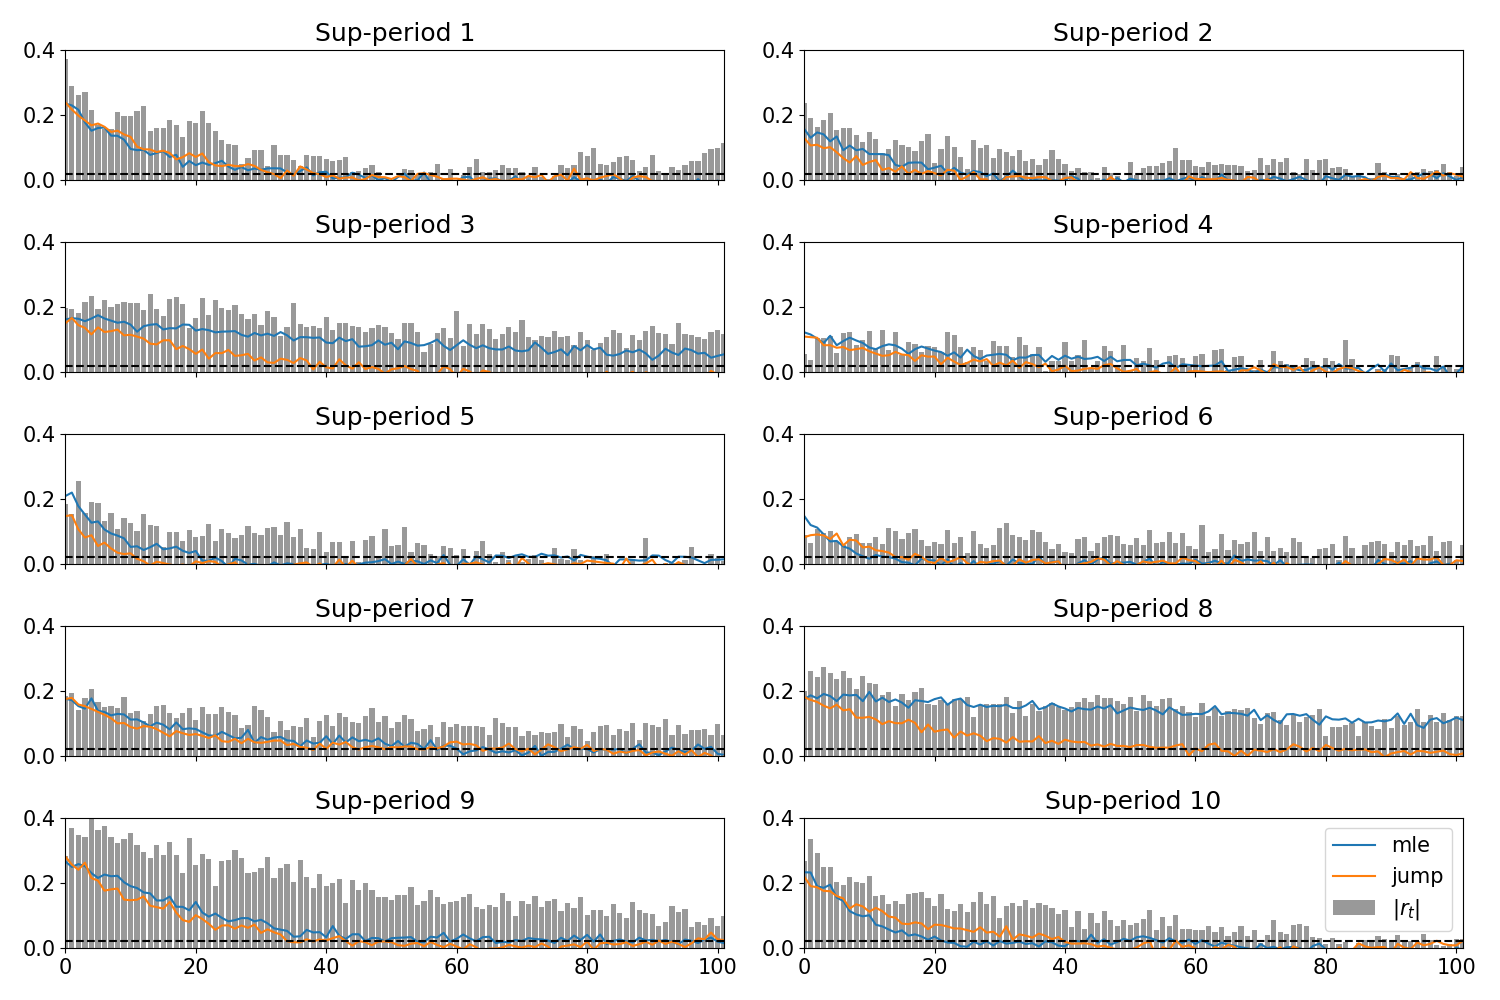
\includegraphics[width=1.0\textwidth]{analysis/stylized_facts/images/acf_abs_subperiods.png}
    \caption{ACf of models and log returns in a breakdown of 10 sub-periods each of 1700 observations.}
    \label{fig:stylized_facts_acf_plots_sub_periods} 
\end{figure}

From the figure, it is evident that the autocorrelation functions estimated directly from the mle and jump model show a much faster decay than the decay of the empirical absolute ACF, thereby confirming the results of both Rýden et al (1998) and Bulla et al. (2011). Despite this property, the autocorrelation function generated by both the mle and jump model, does capture the general tendency of the empirical absolute ACF reasonably well, with the exception of the models in sub-period 9 and 10. However, it also appears that the jump model provide a better fit compared to the model which is estimated through the mle approach. This is in line with the fact that Bulla et al. (2011) concluded that t-distributed HMMs estimated by the mle approach provide a superior fit compared to a traditional Gaussian HMM. Even though the thesis neglect the fitting of a t-distribution, the general conclusion that constraining the models either through distributional properties or jump penalizers provide a better fit holds. The neat aspect associated with splitting the the observations of the full sample absolute autocorrelation of the log returns into smaller digestable sub-periods is that the time-varying nature of the absolute autocorrelation of the empirical log returns becomes visible. As such, it appears that the long memory property associated with financial returns is better captured by splitting the full sample data into sub-periods, which in this case is 10. As such, figure \ref{fig:stylized_facts_acf_plots_sub_periods} points towards a similar conclusion as figure \ref{fig:stylized_facts_acf_plots}, since both the mle and jump methodology, in general, reproduces volatility clustering quite well. However, there are periods in which the models, and their associated parameters, fail to fit the absolute ACF of the log returns, which could be due to the models being miss-specified for some time-periods due to the rolling estimation procedure as argued for figure \ref{fig: MLE estimation rolling parameters} and \ref{fig: Jump estimation rolling parameters}. 

% Comment for the large series
 In order to get an overview for the full sample period figure \ref{fig:stylized_facts_acf_plots} plots the full sample empirical absolute autocorrelation function together with the simulated absolute ACF functions of the mle and jump model. The dashed line is the upper boundary of the 95\% confidence interval under the null hypothesis of independence (Madsen, 2008). Furthermore, given the findings from section \ref{Sec: rolling estimation}, which highlighted the impact that outlier observations had on the estimation procedure, the second plot in figure \ref{fig:stylized_facts_acf_plots} contain the outlier adjusted absolute autocorrelation function of the log returns generated from the S\&P500 index. As such, values outside the interval $\Bar{r_t}\pm 4\hat{\sigma}$, where $\Bar{r_t}$ and $\hat{\sigma}$ are the estimated sample mean and standard deviation, are removed. Granger \& Ding (1995b) proposed setting the observation that are more than 4 standard deviations away from the mean equal to the nearest boundary, however, given the analysis and conclusions of section \ref{Sec: rolling estimation}, removing the outliers is deemed more appropriate. 

Furthermore, according to Granger et al. (2000) the choice of making the cut-off at four standard deviations was arbitrary, but later experimentation and analysis concluded that the results were not
substantially altered if the value was changed slightly. Nevertheless, the long memory of the absolute autocorrelation is evident from both plots in figure \ref{fig:stylized_facts_acf_plots} even though the omission of a large number of exceptional observations greatly reduces the magnitude of the absolute ACF of the outlier limited returns. Furthermore, the reader should note that the persistence of the ACF of the absolute returns is, to some extent, both for the full sample and the outlier adjusted, a consequence of the aforementioned volatility clustering, however, the significant level of the lags above lag 100 is more likely a result of the data-generating process being nonstationary (Nystrup, 2017). 

\begin{figure}[H] 
    \centering
    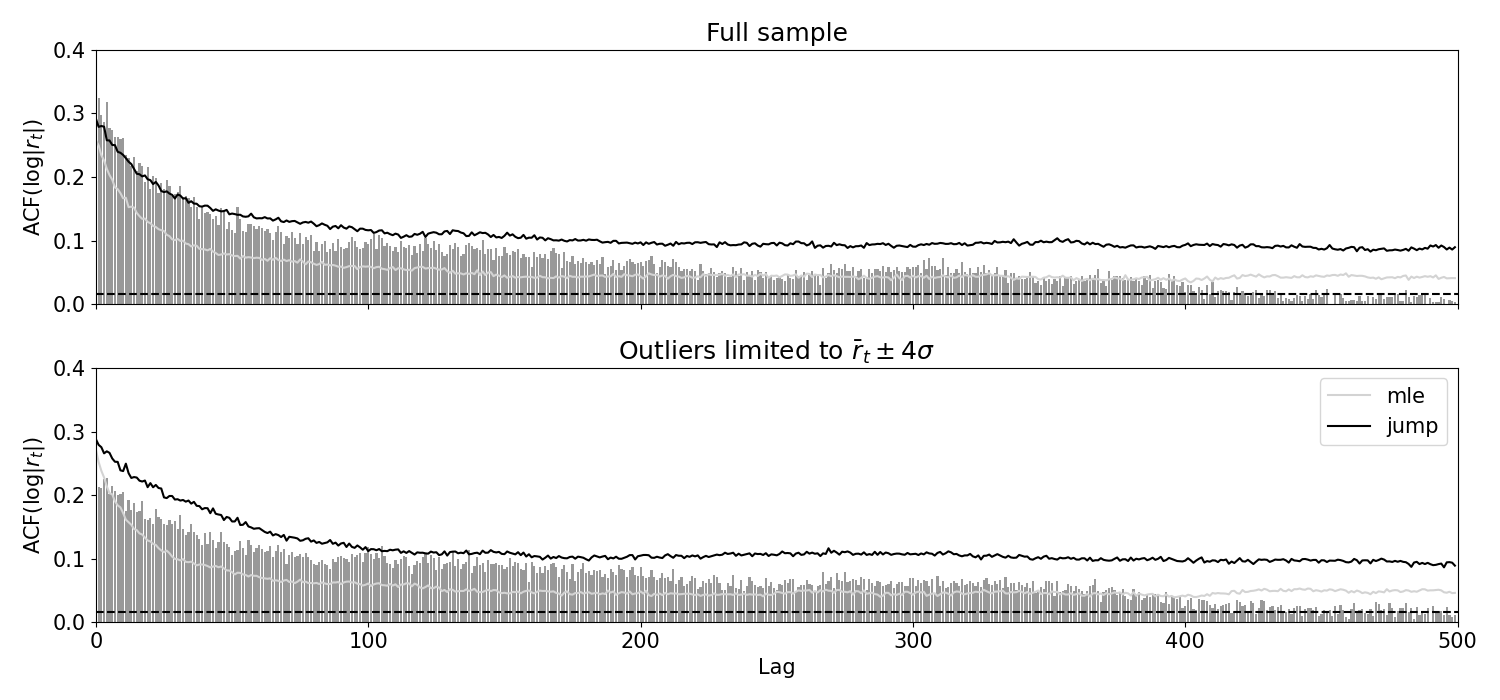
\includegraphics[width=1.0\textwidth]{analysis/stylized_facts/images/acf_abs_models.png}
    \caption{ACF of models as well as log returns.}
    \label{fig:stylized_facts_acf_plots} 
\end{figure}

From the plot in figure \ref{fig:stylized_facts_acf_plots} it is evident that that jump approach does a better job at reproducing the shape of the absolute ACF for the first 200 lags, however, the mle procedure obtains a better fit for lags above 200. Particularly, the jump model decays more slowly, which is evident by the increasing gap between the mle and jump models. In addition, it was shown by Bulla et al. (2011) that increased persistence was achieved as the level for excess kurtosis increased. This allowed for fewer state changes, and hence explains the pattern in figure \ref{fig:stylized_facts_acf_plots}. Interestingly, the mle model displays less absolute autocorrelation than the absolute empirical ACF, however, the jump model displays higher absolute autocorrelation compared to the absolute empirical ACF. As such, neither of the models reproduce the long memory associated with financial returns. In addition, neither of the model's absolute autocorrelation become insignificant, which is in-line with the actual autocorrelation of the absolute empirical ACF. The reader should note, that since the computation underpinning the autocorrelation plots of figure \ref{fig:stylized_facts_acf_plots} relies on simulations, the true autocorrelations are probably higher, as the bouncing behaviour from simulations exhibited in figure \ref{fig:stylized_facts_rolling_moments_outliers}, should reduce autocorrelation. Future analysis should be conducted to uncover whether the autocorrelation can be reproduced more accurately, for instance by increasing excess kurtosis or through modelling the sojourn times through exponentially decaying weights in order to improve persistence in the model estimation procedure (Nystrup et al., 2017).

The remaining stylized fact is TP3, which is often referred to as the Taylor effect. In order to analyse whether the Taylor effect holds, the coefficient $\theta$ is estimated for every period by maximizing the first order autocorrelation of $|r_t|^{\theta}$. The estimation relies on the approach of Rýden et al. (1998) in which the value of $\theta$ maximizing the first order autocorrelation for the models was estimated over the range {0.1 - 2.0} through Monte-Carlo simulation. 

\begin{figure}[H] 
    \centering
    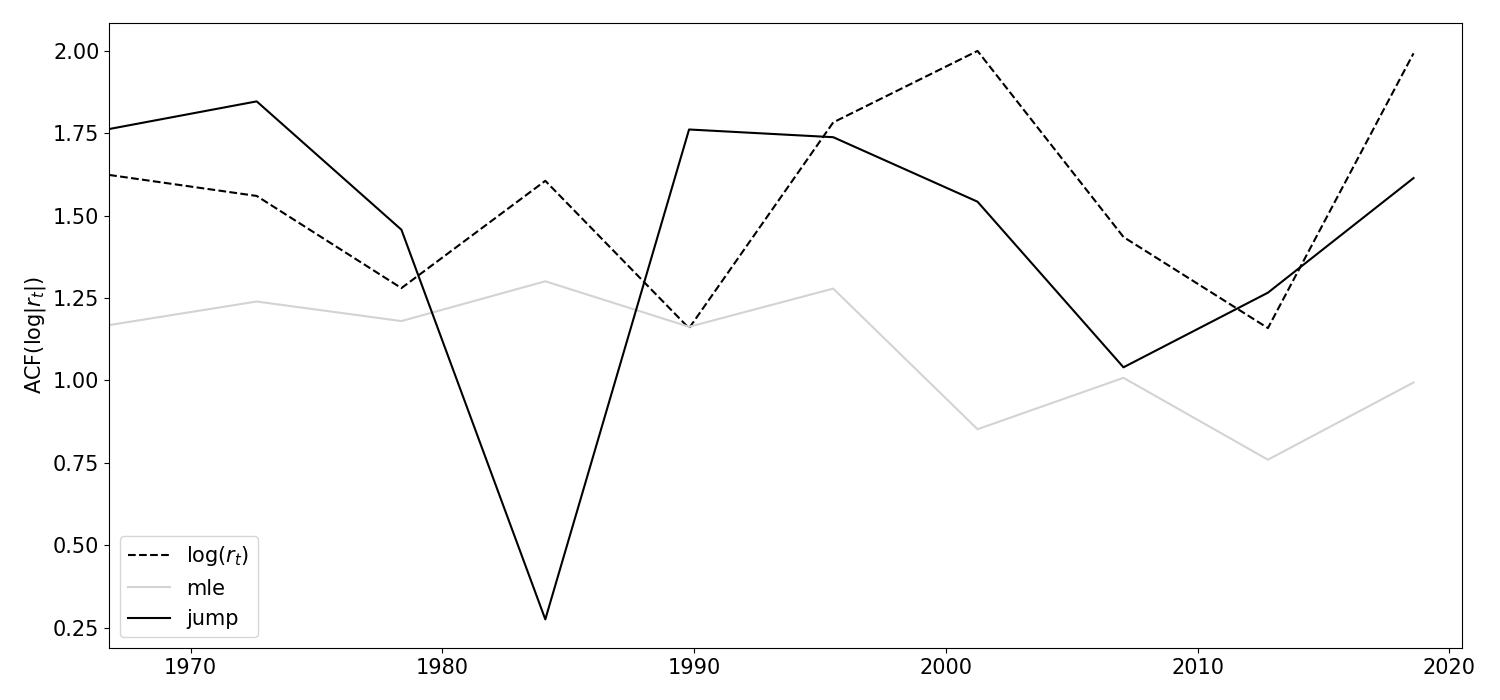
\includegraphics[width=1.0\textwidth]{analysis/stylized_facts/images/acf_taylor_effect.png}
    \caption{Taylor effect. Comparison of the $\theta$ maximizing first order autocorrelations of the data as well as for the models. It is computed by Monte-Carlo simulations and subsequent use of numerical maximization.}
    \label{fig:stylized_facts_taylor_effect} 
\end{figure}

Figure \ref{fig:stylized_facts_taylor_effect} summarizes the results. On the
one hand, maximizing values of $\theta$ for the data series are are not exactly equal to 1, thereby suggesting that neither models fully captures the properties stipulated by TP3. The jump model varies a lot throughout the period and never fully stabilizes at a level of 1 as stipulated by TP3. Furthermore, the values for the model that is generated based on the mle approach achieves a decent fit from 1980 to 1990, and even during the GFC and recent COVID-19 recession it achieves a decent fit very close to 1.


\subsection{Distributional properties}
\label{Sec: Distributional properties}
The previous section performed an in-depth analysis of the temporal properties, yet in order to provide the reader with an overview of how the four moments behave across time as well as the models' ability to capture them, figure \ref{fig:stylized_facts_rolling_moments} plots the empirical moments of the S\&P 500 log returns and the two state Gaussian HMM estimated by the mle and jump approach. At each time $t$, the first four moments are computed using a rolling window of 1700 days.

\begin{figure}[H] 
    \centering
    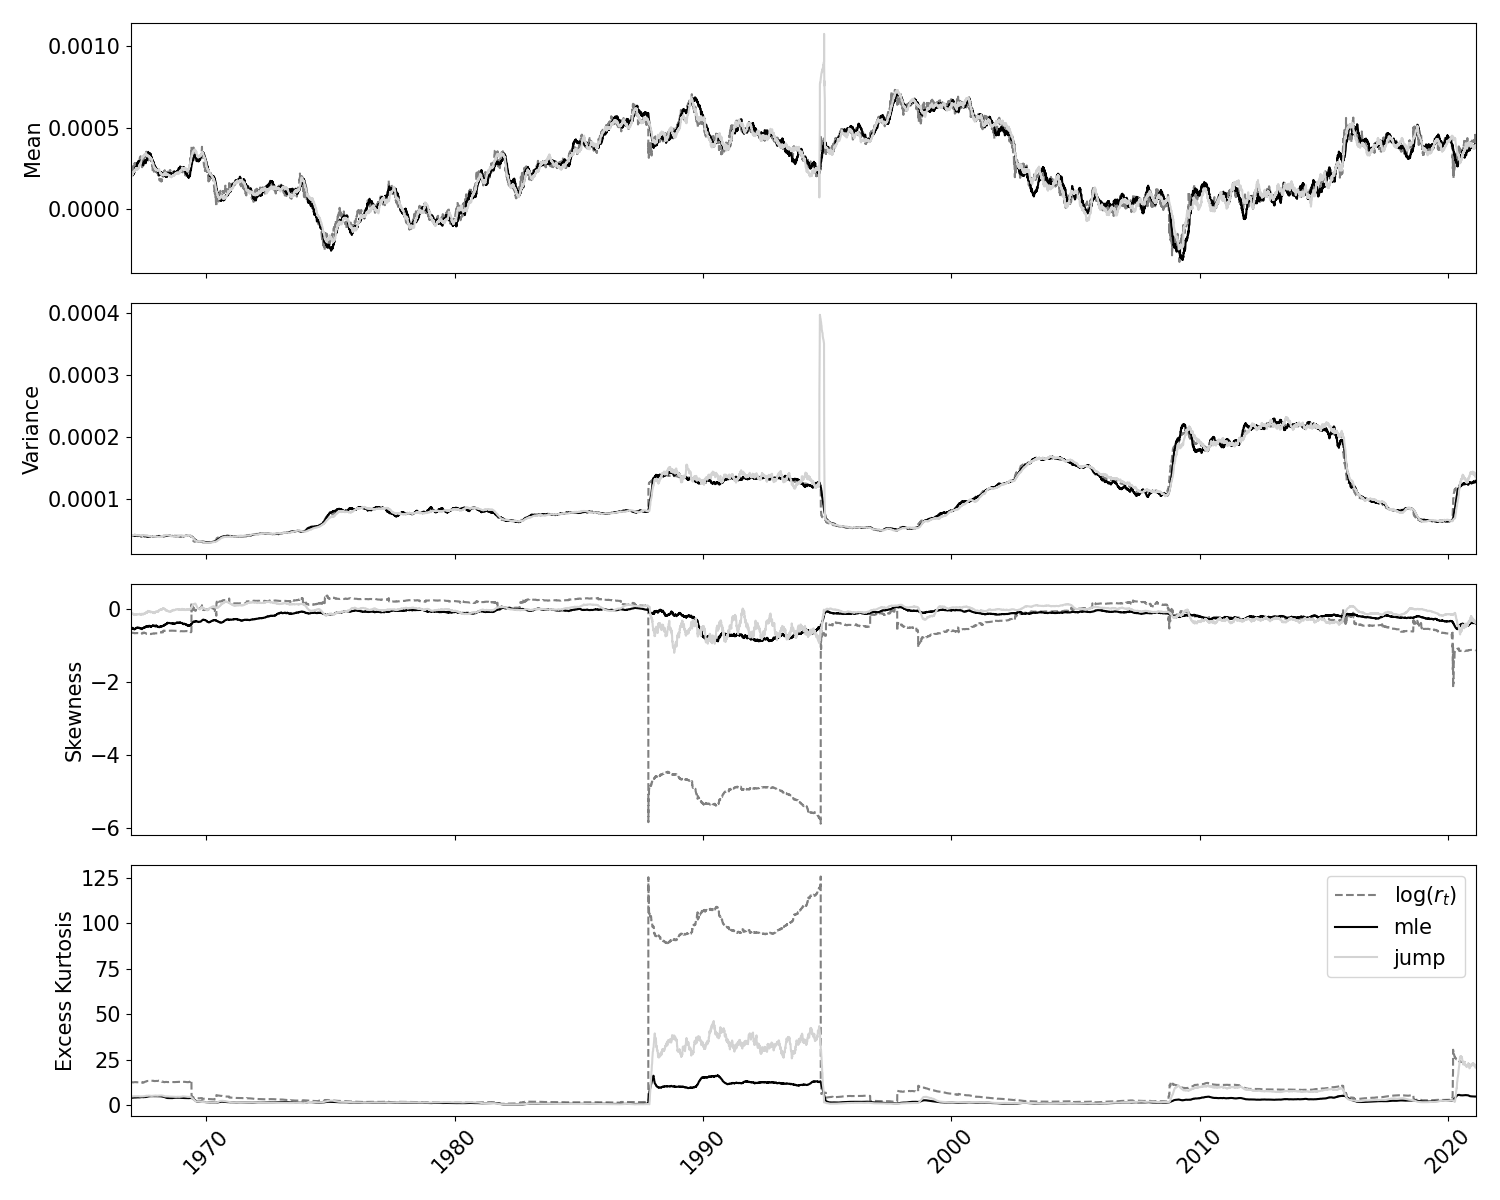
\includegraphics[width=1.0\textwidth]{analysis/stylized_facts/images/rolling_moments.png}
    \caption{Development of first four moments of estimated models compared to $\log(r_t)$ using a rolling window of 1700 days. Model estimates are calculated using Monte-Carlo simulations.}
    \label{fig:stylized_facts_rolling_moments} 
\end{figure}

When analysing figure \ref{fig:stylized_facts_rolling_moments} it is evident that both the mle and jump model are able to reproduce the first two moments quite well, since the mean and variance matches that of the empirical data across time. However, as explained in section \ref{section: Data}, the properties of log returns are not captured by a traditional Gaussian distribution, which is also evident by figure \ref{fig:stylized_facts_rolling_moments}. Particularly when analysing the skewness and kurtosis both the mle and jump model fail short of matching the levels of the empirical distribution. This is evident during periods of high market volatility, for instance during Black monday in 1987 and more recently the COVID-19 recession since the skewness of the log returns drops from a fluctuating level around 0 to -6 and -2 respectively. This suggest that more observations fall into the left part of the distribution thereby suggesting periods of low returns. The same conclusion is apparent for the excess kurtosis since the excess kurtosis of the log returns increases dramatically during periods of high market volatility and both the mle and jump model fails to reproduce this at a satisfying level. The problem can be explained by a few factors. Firstly, Bulla et al. (2011) showed that fitting an HMM through the mle framework based on a conditional t-distribution rather than a conditional Gaussian distribution in the high-volatility state significantly increased excess kurtosis. Secondly, Nystrup et al. (2017) showed that having exponentially decaying weights, thereby reducing the impact of older observations, would improve the fit of the models. Nevertheless, even a Gaussian HMM based on the simplistic mle and the slightly more complex jump procedure can capture big variations in returns, thereby showcasing some model adequacy.

Furthermore, the time-varying nature of the four moments in figure \ref{fig:stylized_facts_rolling_moments} further cements the appropriateness in using rolling estimations. However, an interesting pattern emerges, particularly evident from the sharp increase in excess kurtosis. As such, the Black Monday event in 1987 had market dropping rapidly, thereby increasing kurtosis significantly. Yet, the following period is also characterised by a high degree of excess kurtosis, despite the fact that markets were much calmer. This is a natural consequence of including the observation of Black Monday in the rolling estimation procedure, hence outlier correction should be considered. Due to these findings figure \ref{fig:stylized_facts_rolling_moments_outliers} have been plotted below. The figure does not show the mean and variance but rather the mean to standard deviation ratio as this is used to analyze DP2. The outlier correction has been done so that observations more than 4 standard deviations away from the mean have been omitted. An identical plot to \ref{fig:stylized_facts_rolling_moments}, where all four outlier corrected moments have been shown can be found in appendix \ref{fig:stylized_facts_rolling_moments_outliers_appendix}. The figure in appendix \ref{fig:stylized_facts_rolling_moments_outliers_appendix} will show that the models are still able to reproduce the first two moments very well.


\begin{figure}[H] 
    \centering
    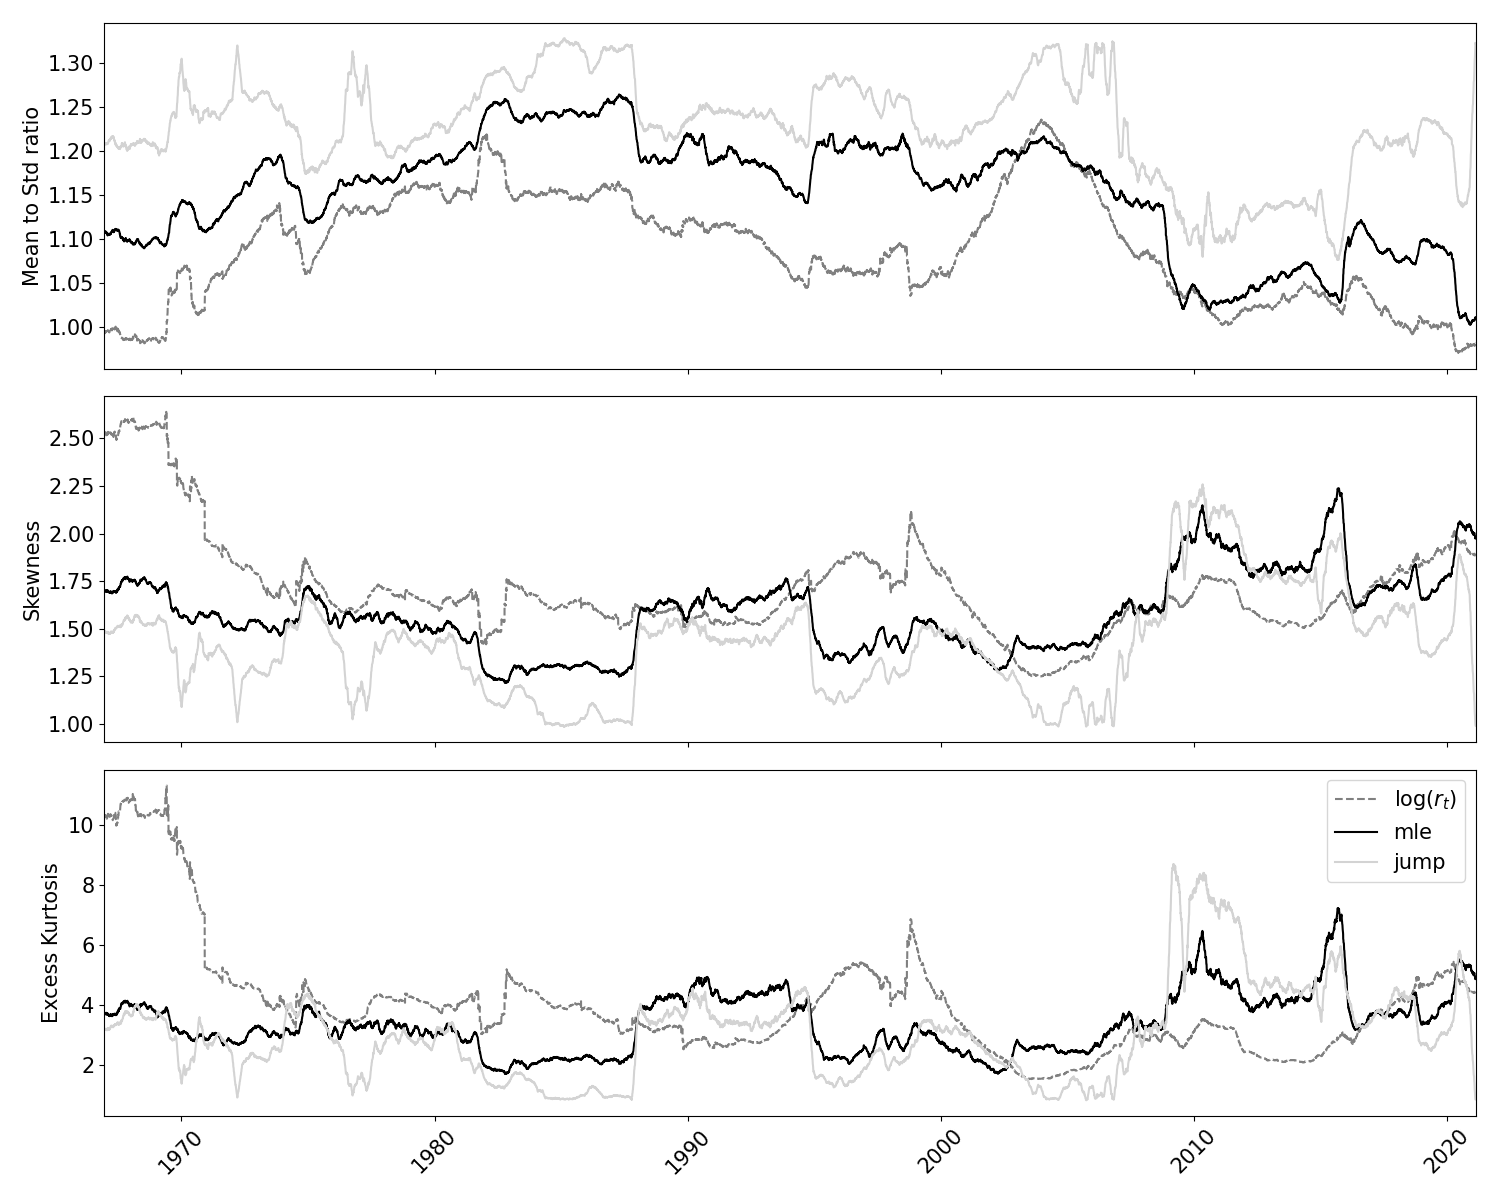
\includegraphics[width=1.0\textwidth]{analysis/stylized_facts/images/rolling_moments_abs.png}
    \caption{Mean to std ratio as well as skewness and kurtosis of $\log(|r_t|)$ and estimated models after outlier correction.}
    \label{fig:stylized_facts_rolling_moments_outliers} 
\end{figure}

It is evident from figure \ref{fig:stylized_facts_rolling_moments_outliers} that removing the outliers have improved both models' ability to capture and reproduce the skewness and excess kurtosis of the empirical distribution. In addition, it appears that both models are still able to capture the changing skewness and excess kurtosis around the time of large market movements, despite removing the outliers. This is evident throughout the figure, but particularly around the time of the GFC. The fact that both models are able to do so is particularly promising as it provides substantial evidence towards the adequacy of the models. The fit of the models could be further improved by calibrating the models as explained above, or by increasing the number of states. However, the problem with the latter option is that it significantly increases the risk of overfitting (Bulla et al. 2011). As noted in the section \ref{subsection: temporal properties}, which touched upon the temporal properties, Granger \& Ding (1995b) also defined as set of stylized facts for distributional properties. These are defined as follows:

DP1: $|r_t|$ and $sign(r_t)$ are independent\newline
DP2: Mean$|r_t|$ = standard deviation $|r_t|$ \newline
DP3: The marginal distribution of $|r_t|$ is exponential (after outlier correction)

In addition, it should be noted that an exponentially distributed variable (DP3) $x_t$ has the following properties.

PED1: $E(x_t) = \sqrt{Var(x_t)}$ (Same as DP2) \newline
PED2: $E[x_t-E(x_t)]^3 / (Var(x_t))^{\frac{3}{2}} = 2.$ \newline
PED3: $E(x_t-E(x_t))^4 / (Var(x_t))^{2} -3 = 6.$

In the analysis conducted by Rýden et al. (1998) and Bulla et al. (2011) it has been proven that DP1 holds as a natural consequence of the construction of HMMs. Despite this, the reader should note that the ratio of the mean and standard deviation i.e. (PED1/DP2) is sometimes slightly overestimated by both models. This property is also in line with the conclusions achieved by Rýden et al (1998) and Bulla et al. (2011), who both noted that PED1 has to be relaxed. This means that the mean has to be allowed to be slightly larger than the standard deviation if PED2 and PED3 are to be satisfied simultaneously.

Moving on to the analysis of DP2 it is clear from figure \ref{fig:stylized_facts_rolling_moments_outliers} that the mean is higher than the standard deviation for the absolute log returns as well as the mle and jump model for the predominant part of the period. Despite this, it appears that neither of the two models sway too far away from 1, thereby indicating that the mean of the absolute returns is approximately equal to the standard deviation of the absolute returns for both models. Furthermore, it is evident by the figure that the mle model in particular converges to 1.0 during the period following the financial crisis as well as the recent COVID-19 recession. A similar pattern is evident for the jump model, although not to the same extent as the mle model. As such, it can be concluded that the ratio of the mean to standard deviation (PED1/DP2) is close to one for all fitted models, although it is sometimes slightly overestimated.

Having analysed whether the models satisfy DP1 and DP2 the final distributional property to consider is DP3. For DP3 to be satisfied the models must exhibit the properties of PED1, PED2 as well as PED3. Since it was just shown that DP2 holds for both models, and PED1 and DP2 is identical in their construction, it can be concluded that PED1 holds for both models. Furthermore, it is evident that both the mle and jump model underestimate skewness in most of the periods, however, it appears that both models achieves a better fit towards PED2 in the period following the financial crisis of 2008. The reader should also note that it is evident from figure \ref{fig:stylized_facts_rolling_moments_outliers} that the mle model better matches the skewness property put forward by PED2 compared to the jump model as well as the empirical data for most of the period. As such, it can be concluded that both models reproduce the stylized facts quite well, although neither model achieve a perfect fit. 

The final property that the models must satisfy in order for DP3 to be met is PED3. As such, the models must be able to exhibit and match an excess kurtosis of 6. It is clear from figure \ref{fig:stylized_facts_rolling_moments_outliers} that both models slightly underestimate the excess kurtosis for the predominant time, however, similar to the observations of the skewness, it appears both models approximately match an excess kurtosis of 6 in the period following the financial crisis of 2008. Furthermore, both models seem to perform equally well on average throughout the period. To summarize the above findings, both the mle and the jump models are able to somewhat reproduce the properties of PED1 to PED3, hence it can be concluded that DP3 holds. This is similar to the conclusion reached by both Rýden et al (1998) and Bulla et al. (2011), although they only tested HMMs estimated through the mle methodology. As such, this thesis contributes to the quantitative finance literature by showcasing that the stylized facts introduced by Granger \& Ding (1995b) can in fact be reproduced by a jump model and not just the traditional HMM estimated through the mle approach. As such, the thesis have extended on the introduction of jump estimation procedure for HMMs by Bemporad el at. (2018) by proving that it matches the properties of the stylized facts associated with returns on financial assets.

\subsection{Decoding and prediction}
As mentioned in section \ref{section: estimation} the hidden states are uncovered through the Viterbi algorithm. Since the estimation procedure is based on a rolling window, the state at time $t$ is estimated by using the most recent observation as well as the previous 1699. As such, the decoding procedure iterates through the entire row of observations 1 time step at a time as shown in figure \ref{fig:stylized_facts_decoded_states}. As previously mentioned, it is important to stress that the objective of this procedure is not to predict future states of the economy, but rather to identify and uncover the current state underlying the economy given past observations. 

\begin{figure}[H] 
    \centering
    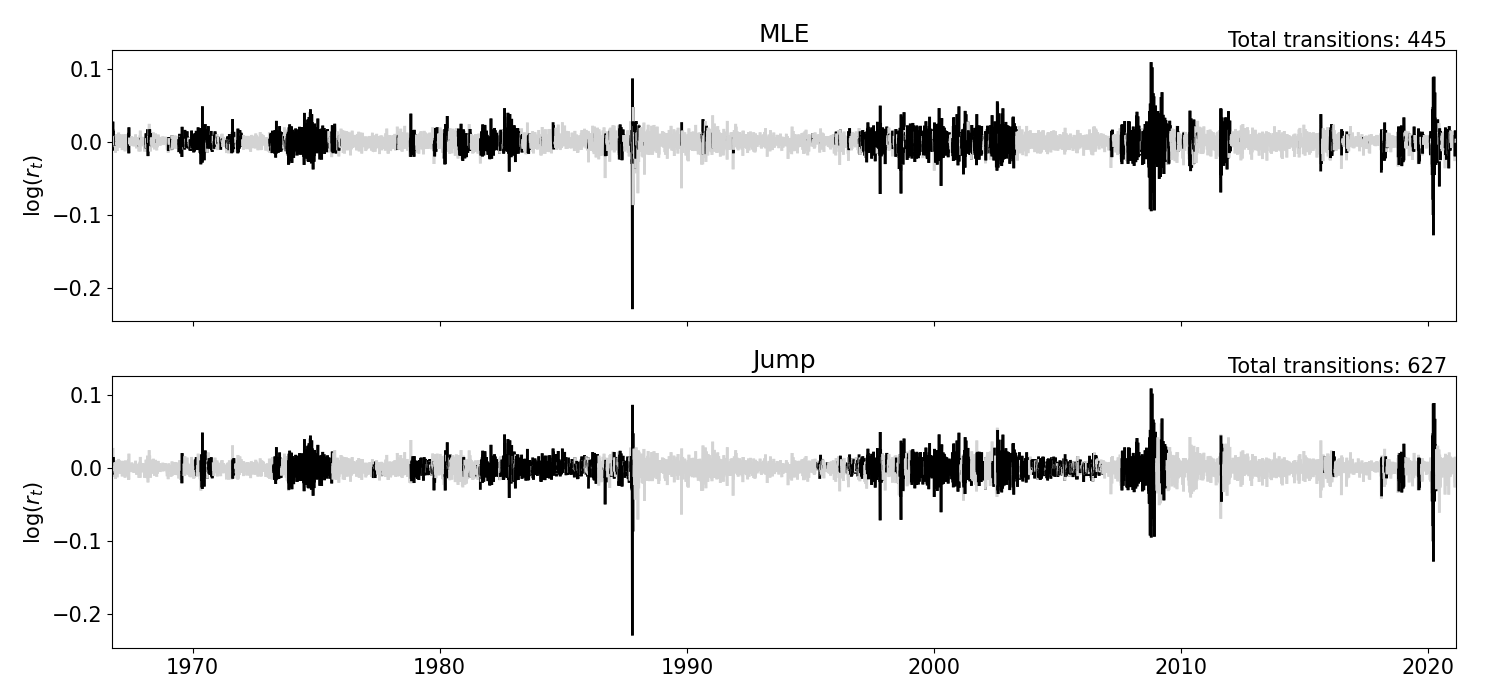
\includegraphics[width=1.0\textwidth]{analysis/stylized_facts/images/decoded_states.png}
    \caption{S\&P 500 log returns plotted with the respective model's decoded states. States are decoded using a rolling window of 1700 trading days. Black indicates the high-variance state.}
    \label{fig:stylized_facts_decoded_states} 
\end{figure}

It is evident from the figure that the mle model does a decent job in detecting the high-volatility states. However, it also appears that the model identifies some high-variance states in periods characterised by low market volatility, for instance in the beginning of the 1990s. This is most likely a result of low excess kurtosis. A similar pattern appears when analysing the decoding states of the jump model since it too does a fairly good job at identifying the high-variance state, although the two methods disagrees in some time periods. This is for instance evident when looking at 1985 to 1990 where the mle models suggests a low variance state, contrary to the jump model. Furthermore, it appears that the jump model is less consistent compared to the mle model as it jumps around more sporadically. This is backed by the fact that the jump model suggests 627 state transitions throughout the period which is more than 40\% more state changes compared to the suggested 445 transitions by the mle model. This is perhaps surprisingly since the jump framework penalizes state transitions, however, this is most likely a result of the rolling estimation approach. As such, if one were to conduct a similar analysis in which the jump model was estimated by batches or on the full sample size, the total suggested transitions would most likely decrease, albeit these estimation procedures would introduce other problems. 

In addition, it is positive to witness that both models correctly identifies major market events such as Black monday in 1987, the dot-com bubble of the early 2000s, the GFC of 2008 and most recently the COVID-19 recession as high-variance states, albeit the models disagree in terms of how long the high-variance state persists. Furthermore, it was evident by figure \ref{fig: SP500_index} that there were short periods of large positive returns following the big market crash in September/October 2008, however, both models predict those as bear states, which indicates that variance dominates means in the prediction of whether a state is classified as high or low variance. Another aspect that has to be considered in terms of using the either model, but particularly the jump, is the cost of changing the portfolio allocation due to a wrong signal. As evident by figure \ref{fig: SP500_index} the period from 1980 to 1990 is characterised by increasing price levels and low variance, hence the correct classification of the state should be low-variance, however, the jump model classifies it as a high-variance state throughout the period. As such, utilising the models when forming DAA strategies should be done carefully, as the amount of transitions and possibly miss-specified states can decrease profits and Sharpe ratios substantially.  

\subsubsection{Smoothing}
In the previous section it became evident that the amount of transitions between the two states are high for both models with the mle and jump model proposing 445 and 627 transitions respectively. This amount of state transitions decreases the confidence that the uncovered state changes occur due to the economy entering a new state, while increasing the suspicion towards random sporadic jumps. Furthermore, it was evident that the jump model proposed more than 40\% more transitions compared to the mle, and this constitutes an issue due to the objective of jump model being to constrain sporadic and frequent jumps. Lastly, such fluctuations and sporadic transitions can be costly in a DAA framework, especially when factoring in opportunity cost of allocating capital poorly due to a miss-specified state, and when factoring in actual trading costs. As a result of these conclusions, a probability smoothing scheme is implemented to improve persistence and hence reduce the amount of state transitions. For every state prediction at time $t$, the probability of being in all states are computed as described in section \ref{section: estimation}. This is then compared to a median threshold hence a state change will only occur if the past 4 out of 7 state predictions suggest that a change must occur. The choice of threshold is a trade-off between the time-delay in state changes and the confidence in state predictions as described by Nystrup (2014). The associated results of applying such a smoothing scheme is shown for the mle and jump model in figure \ref{fig:stylized_facts_decoded_states_filtered}.

\begin{figure}[H] 
    \centering
    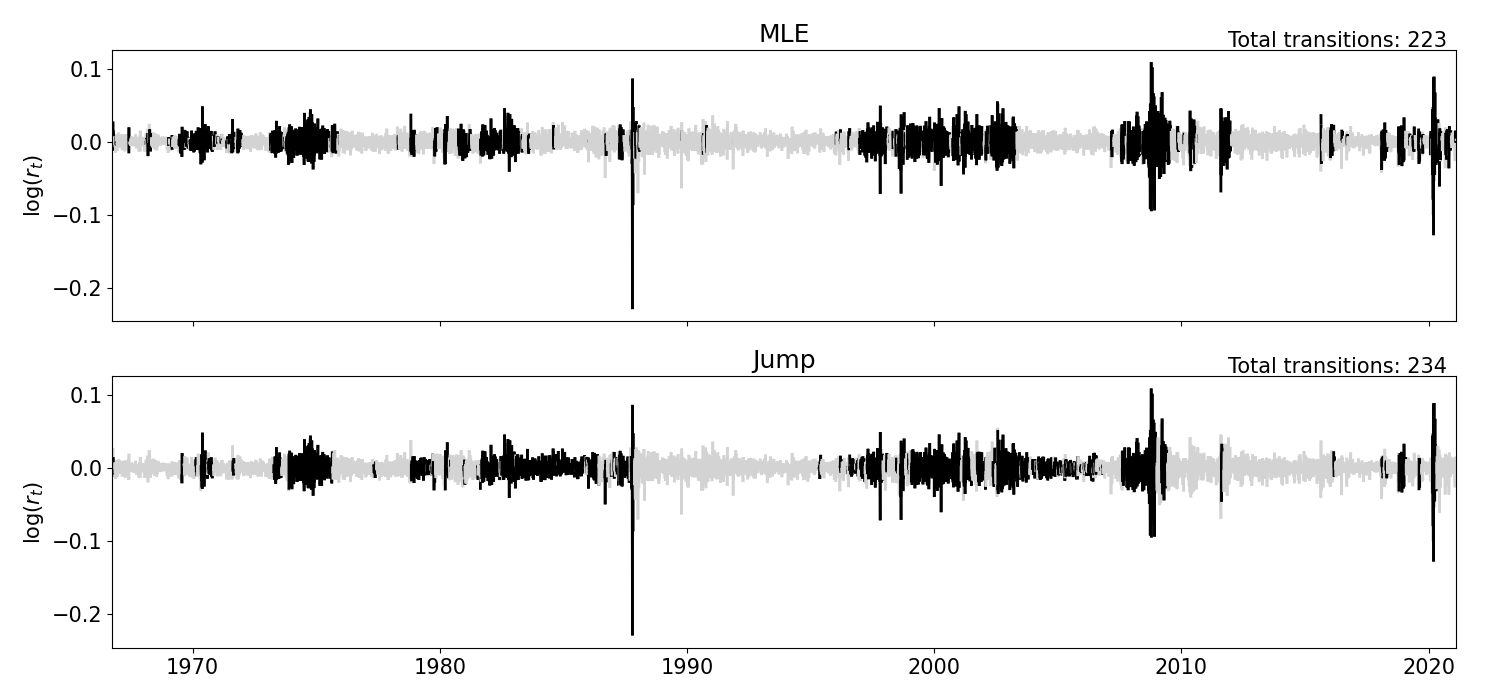
\includegraphics[width=1.0\textwidth]{analysis/stylized_facts/images/decoded_states_filter.png}
    \caption{S\&P 500 log returns plotted with the respective model's decoded states. States are decoded using a rolling window of 1700 trading days.  Black indicates the high-variance state.}
    \label{fig:stylized_facts_decoded_states_filtered} 
\end{figure}

It is evident that the number of proposed transitions reduces dramatically from 445 to 223 for the mle model and from 627 to 234 for the jump model. The drastic decrease in transitions is primarily visible in the fewer amount of short-lived sojourn times. However, despite the apparent decrease in the number of transitions, there still appears to be inconsistency across the two models in terms of state predictions. This is once again evident in the time period from 1985 to 1990 in which the mle model suggests low-variance states and the jump model suggests high-variance states. Yet, both models are still able to capture the big market events as previously described. Furthermore, applying the probability smoothed models serve as a better option compared to the non-smoothed alternative in a DAA framework since the reduction in state transitions, all else equal, will reduce trading costs and increase returns. 

As conclusively remarks of section \ref{Section: Stylized facts}, it appears that both the mle and jump model are able to reproduce the four temporal as well as the three distributional properties, however, the jump model does an overall better job. Particularly, when reproducing the empirical absolute autocorrelation function the jump model achieves a better fit for the first 200 lags, although the mle achieves a better fit for the remaining lags. Furthermore, there is a significant variation in the parameters over time, thereby greatly supporting the use of rolling estimation. In addition, the use of rolling estimation has the property that no foresight is assumed at any point in time, thereby making the prediction model likely to generalize well to new data. Lastly, a smoothing scheme has been applied when uncovering the hidden states, thereby increasing state persistence while reducing the amount of transitions between states. Despite these initiatives, it is clear that the models still provide inconsistent state predictions thereby increasing the risk of making poor capital allocation decision, and as a result encounter decreasing profits through a DAA framework. In the following sections, the MPC framework will be introduced and based on this it will be investigated whether trading strategies conditional on the predicted states are profitable.
